% based on sparxHub/Professional_LaTeX_CV.md
% https://www.overleaf.com

\documentclass[10pt,A4]{article}
\usepackage[utf8]{inputenc}
\usepackage{xstring, xifthen}

% FONT BASICS
\usepackage[default]{raleway}
\renewcommand*\familydefault{\sfdefault}
\usepackage[T1]{fontenc}
\usepackage{moresize}

% PAGE LAYOUT
\usepackage{paracol}
\usepackage[a4paper]{geometry}
\geometry{top=1cm, bottom=1cm, left=1cm, right=1cm}

% COLORS
\usepackage{color}
\definecolor{maincol}{RGB}{74, 74, 74}
\definecolor{darkcol}{RGB}{44, 44, 44}
\definecolor{lightcol}{RGB}{245, 245, 245}

\usepackage{graphicx}
\usepackage{hyperref}
\hypersetup{colorlinks=true, urlcolor=darkcol}

% CV COMMANDS
\newcommand{\cvsection}[1] {
    \vspace{14pt}
    {\raggedright\textbf{\LARGE{\textcolor{darkcol}{\uppercase{#1}}}}}\\
    \textcolor{maincol}{ \rule{0.1\linewidth}{2pt} } \\
}

\newcommand{\cvevent}[8] {
    \textbf{#2}%
    \ifthenelse{\isempty{#8}}{}{ {\normalfont\small (#8)}}%
    \hfill \colorbox{maincol}{\textcolor{white}{#1}} \\
    \textcolor{maincol}{\textbf{#3}} \\
    \ifthenelse{\isempty{#4}}{}{\textcolor{darkcol}{#4}\\}
    \ifthenelse{\isempty{#5}}{}{\vspace{5pt}\begin{itemize}#5\end{itemize}}
    \ifthenelse{\isempty{#6}}{}{\vspace{2pt}\hspace{\leftmargini}\textit{#6}\\}
    \ifthenelse{\isempty{#7}}{}{\vspace{5pt}\textbf{Achievements include:}\\\begin{itemize}#7\end{itemize}}
    \vspace{14pt}
}

\newcommand{\cvskill}[3] {
    \textbf{#1} \hfill {#2}\\
    \textcolor{maincol}{\rule{#3\linewidth}{2pt}}\\
}

% DOCUMENT
\begin{document}

\columnratio{0.31}
\setlength{\columnsep}{2.2em}
\setlength{\columnseprule}{4pt}
\colseprulecolor{lightcol}

\begin{paracol}{2}

% LEFT COLUMN
\begin{leftcolumn}

% PROFILE IMAGE
\vspace{10pt}
\begin{center}
    \fbox{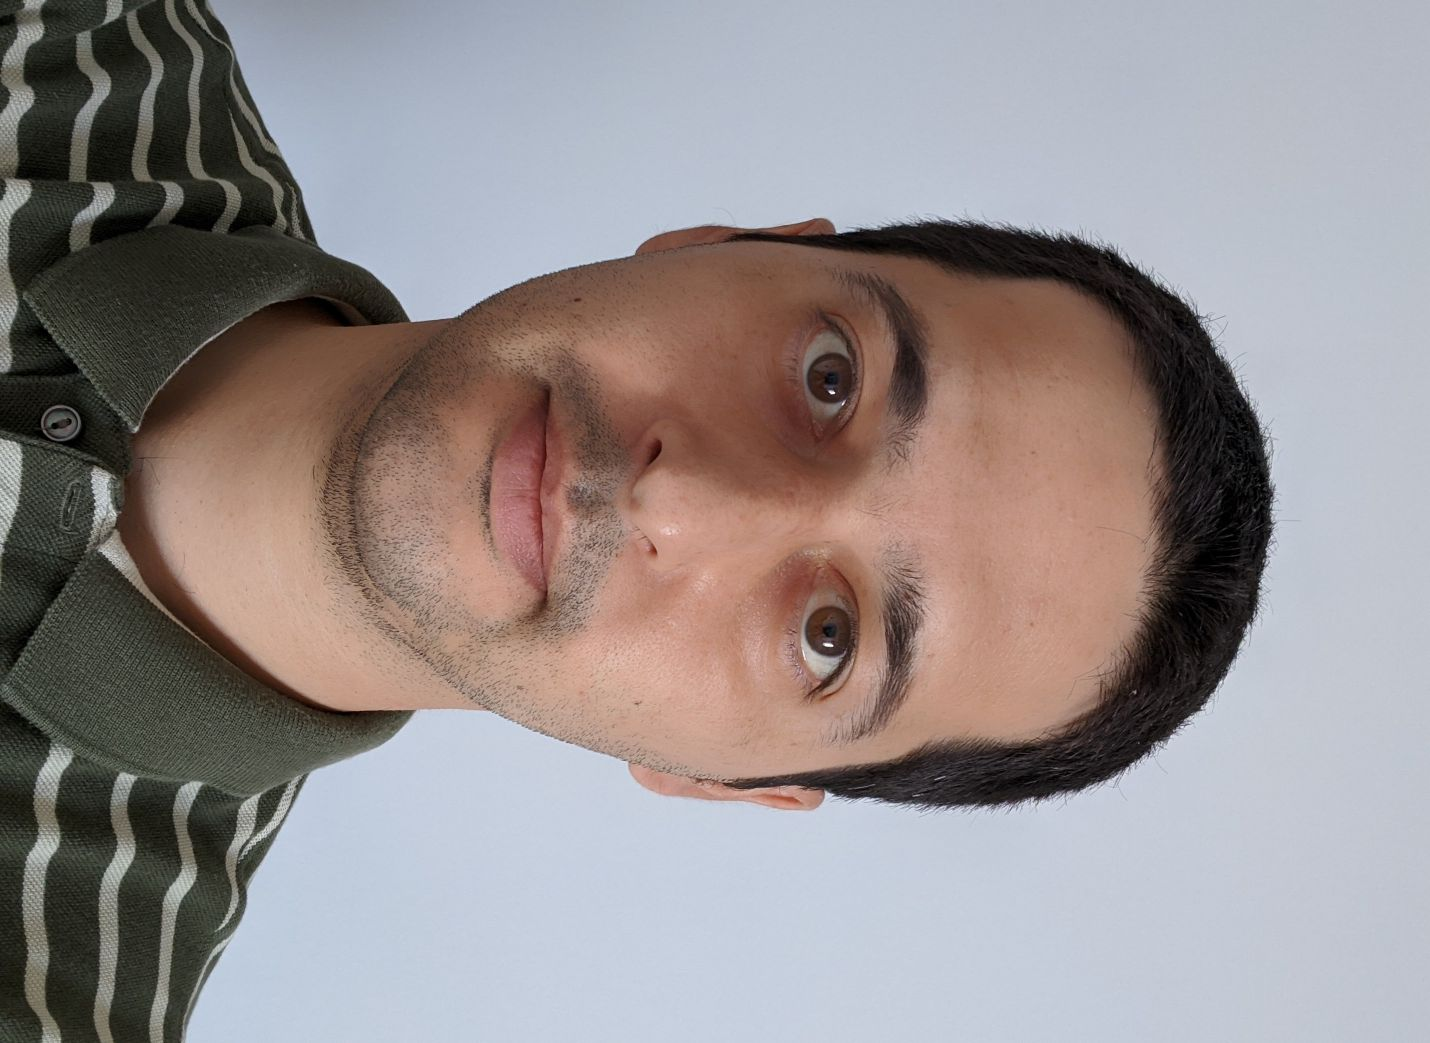
\includegraphics[width=0.9\linewidth, angle=90]{profile.jpg}}
\end{center}
\vspace{10pt}

% CONTACT
\cvsection{CONTACT}
\raggedright
{\LARGE\textbf{Nikolas Pattakos}}\\
\vspace{4pt}
\textit{Software engineer}\\
\vspace{8pt}
France\\
+33  6 61 60 97 53\\
+30 69 45 15 17 20\\
\href{mailto:pattakosn@fastmail.com}{pattakosn@fastmail.com}\\
\vspace{10pt}

% SKILLS
\cvsection{SKILLS}

\cvskill{C / C++}{15+ years}{1.0}
\cvskill{Linux \& kernel}{10+ years}{1.0}
\cvskill{HPC / Parallel (OpenMP, CUDA, MPI)}{10+ years}{1.0}
\cvskill{Qt / GUI}{7 years}{0.9}
\cvskill{Embedded / Yocto}{4+ years}{0.6}
\cvskill{Agile / SCRUM / SAFe}{7+ years}{0.8}

\vspace{6pt}
\textbf{Languages:} C, C++, Python, Bash, Fortran\\
\textbf{Frameworks:} Qt 5/6, OpenMP, CUDA, MPI\\
\textbf{Tools:} CMake, Git, GitLab, Jenkins, gdb, valgrind, perf, gprof\\
\textbf{Libraries:} BLAS / LAPACK, Eigen, Intel MKL\\
\textbf{Domains:} Numerical simulation, 3D / CAD / CAE, Linux/embedded, GPGPU\\
\vspace{10pt}

% LANGUAGES
\cvsection{LANGUAGES}
Greek: Native\\
English: Fluent\\
French: DELF B2\\
\vspace{10pt}

% EDUCATION
\begin{minipage}[t]{\linewidth}
\cvsection{EDUCATION}

\textbf{MSc, High Performance Computing}\\
University of Edinburgh / EPCC, 2008\\
\textit{\small Thesis: ``Derived Metrics with Paraver using hardware counters on Power5 chips''.}\\
\vspace{6pt}

\textbf{BSc, Applied Mathematics}\\
University of Crete, 2007\\
\textit{\small Numerical analysis, linear algebra, solid and fluid mechanics, computer science.}\\
\vspace{6pt}

\textbf{MSc, Electronic \& Computer Engineering \textit{(incomplete)}}\\
Technical University of Crete (TUC), 2008\\
\textit{\small Completed coursework toward an MSc at TUC (3D computer graphics, GPGPU/CUDA, machine learning) but did not submit the dissertation; degree not held. Course projects included a CUDA-accelerated GIS algorithm in MATLAB and an oil-reservoir simulation ported from MATLAB to multi-threaded C ($\sim$8x on dual quad-core) and then to CUDA ($\sim$5.5x further on a GTX~280).}\\
\vspace{10pt}
\end{minipage}

\end{leftcolumn}

% RIGHT COLUMN
\begin{rightcolumn}

% PROFILE
\cvsection{PROFILE}
Senior C++ software engineer with 15+ years across embedded Linux, HPC, and Qt application development, and a strong mathematics background. I deliver and optimise production code at every level of the stack --- from kernel drivers and Yocto-based BSPs, through Qt 5/6 desktop and instrument-control applications, to OpenMP/MPI/CUDA simulation codes running on clusters. Track record of measurable performance gains (2x--5500x on real workloads), diagnosing complex low-level issues, and of delivering in Agile/SAFe environments alongside multinational teams. Trilingual: Greek (native), English (fluent), French (DELF B2).\\
\vspace{6pt}

\cvsection{WORK EXPERIENCE}

% --- Roles inside paracol: these sit alongside the sidebar on page 1.
% --- TUNING THE PAGE 1 BREAK:
% ---   * If the right column ends well above the bottom of the sidebar,
% ---     move the next \cvevent up into this block.
% ---   * If the right column overflows past the sidebar's bottom (forcing
% ---     an empty sidebar onto page 2), move one \cvevent down past
% ---     \end{paracol} below.

\cvevent
{Jun 2025 -- Present}
{Software Engineer}
{Analog Way \textit{(audiovisual hardware manufacturer)}}
{C++, Qt and embedded Linux development on professional video equipment.}
{\item Develop backend services and Linux-side glue connecting web-based control UIs to microcontroller subsystems.
 \item Containerised existing applications with Docker and modernised CI/CD pipelines to run on container-based runners.
 \item Contribute fixes and new features across the product line.
 \item Embedded Linux work on Yocto / BSP-based systems.
}
{C++17, Qt, Yocto, Linux kernel, device tree, Docker, CI/CD, GitLab}
{}
{CDI}

\cvevent
{Mar 2021 -- Jun 2025}
{Software Engineer}
{Thermo Fisher Scientific \textit{(scientific instrumentation)}}
{Contributed to Velox, a C++/Qt application controlling electron microscopes, as part of a distributed team spanning several countries.}
{\item Worked across both UI (Qt views, controls, widgets) and backend (instrument communication, data flow) of a complex scientific-instrument control application.
 \item Worked within a heavily templated, modern C++17 codebase using established GUI architecture patterns (MVP/MVC/MVVM family).
 \item Delivered features and fixes within an Agile/SAFe release-train environment alongside distributed teams.
}
{C++17, Qt, GUI architecture patterns, Agile, SAFe}
{}
{CDI}

\cvevent
{Nov 2020 -- Mar 2021}
{C++ Developer}
{FORTHNET \textit{(Greek telecoms / IPTV / energy)}}
{Maintained and extended the in-house C++ billing system for a major Greek telecom operator.}
{\item Bug fixes and small features on a multi-threaded C++ / Oracle SQL billing system.
}
{C/C++, Linux, Oracle SQL, multithreading}
{}
{CDI}

\begin{minipage}[t]{\linewidth}
\cvevent
{Nov 2019 -- Nov 2020}
{Software Engineer}
{CNRS \textit{(astrophysics research laboratory)}}
{Performance and parallelisation work on a production C++/Fortran atmospheric simulation code (MPI + OpenMP) at a CNRS astrophysics laboratory.}
{\item Profiled and optimised hot paths in a long-running simulation codebase, improving its scalability for new simulation campaigns.
 \item Ran and managed large-scale jobs on Slurm-managed Linux clusters; automated pre/post-processing pipelines in bash and Python.
}
{C++11, Fortran, OpenMP, MPI, Slurm, Bash, Python, HPC}
{}
{CDD}
\end{minipage}

\cvevent
{Oct 2018 -- Dec 2018}
{Software Engineer}
{AKKA Technologies \textit{(consulting)}}
{Profiled and optimised an Unreal Engine 4 automotive HMI/cockpit visualisation scene to lift its frame rate.}
{\item GPU-side performance work across the rendering pipeline --- draw-call profiling, render-pass analysis, shader-cost reduction --- driven by bottleneck analysis at both engine and project-blueprint level.
 \item Nearly \textbf{2x frame rate}, reaching the limit set by the project's blueprints.
}
{Unreal Engine 4, C++, GPU profiling, real-time rendering}
{}
{CDI}

\end{rightcolumn}

\end{paracol}

% FULL-WIDTH CONTINUATION
% From here onwards the sidebar is closed and content flows the full page width.

\cvevent
{Mar 2017 -- Sep 2018}
{Software Engineer}
{INRIA \textit{(applied mathematics research laboratory)}}
{Contributed to ParMMG, the MPI-parallel version of the open-source MMG mesh-adaptation library (\href{http://www.mmgtools.org}{mmgtools.org}), at INRIA's applied-mathematics laboratory.}
{\item C/C++ development on the parallel re-meshing algorithms and surrounding infrastructure.
 \item Bug fixes, automated unit-test development, and maintenance of the project's Jenkins/Apache CloudStack CI system.
}
{C, C++, MPI, OpenMP, CMake, Git, Jenkins, Apache CloudStack}
{}
{CDD}

\cvevent
{Mar 2015 -- Mar 2017}
{Software Engineer}
{INRIA \textit{(applied mathematics research laboratory)}}
{Performance and reliability work on multiple HPC simulation codes (C, C++/CUDA, Fortran) at INRIA's applied-mathematics laboratory, in collaboration with researchers and PhD students.}
{\item Algorithmic redesign delivered up to \textbf{5500x speedup} on individual compute kernels, with \textbf{2x--4x} end-to-end gains across whole simulations.
 \item \textbf{Reduced} simulation \textbf{memory} footprint by \textbf{20--50\%} via \textbf{data-structure optimisation}.
 \item Bug fixes, automated unit-test development, and maintenance of the lab's CI infrastructure (Jenkins / Apache CloudStack).
 \item Operated jobs on Slurm-managed Linux clusters; orchestration and post-processing in bash and Python.
}
{C, C++, CUDA, Fortran, MPI, OpenMP, Jenkins, Apache CloudStack, Slurm, HPC}
{}
{CDD}

\cvevent
{Nov 2013 -- Mar 2015}
{System Administrator \& Operations Engineer}
{HCMR \textit{(biology research institute)}}
{Sole administrator of HCMR's HPC Linux cluster supporting biology and genetics research; also operations support for the institute's web developers.}
{\item Owned the cluster end-to-end: designed and led its upgrade to 600 cores, InfiniBand interconnect, and a $\sim$200~TB Lustre parallel file system.
 \item Built an automated multi-server backup system based on BACULA.
 \item Provided dev/ops support to web developers across a stack including Drupal, Tomcat, PostgreSQL, R, and QEMU/VirtualBox VMs --- including for the X-ray 3D image-reconstruction component of \href{http://www.lifewatchgreece.eu}{lifewatchgreece.eu}.
 \item Implemented an internal C++/CUDA/Qt utility (using GMP for arbitrary-precision arithmetic) computing biological indices from CSV input.
}
{Linux, HPC, Lustre, InfiniBand, BACULA, QEMU, VirtualBox, Drupal, Tomcat, PostgreSQL, R, C++, CUDA, Qt, GMP}
{}
{CDD}

\cvevent
{Feb 2012 -- Jul 2013}
{Software Engineer}
{Imagination Technologies \textit{(semiconductor design)}}
{Kernel-mode driver and firmware development on the PowerVR 3D graphics IP, working within Imagination's GPU driver team.}
{\item Bug fixes and feature work across kernel-mode driver (KMD) code and on-GPU firmware.
 \item Software-side bring-up and validation against simulators and dev boards.
 \item Multi-platform targets: Android, Linux, and Windows Mobile.
}
{C, Linux kernel, KMD, GPU firmware, Android, Windows Mobile, Perforce}
{}
{CDI}

\cvevent
{Feb 2009 -- Nov 2009}
{Software Engineer}
{HCMR \textit{(biology research institute)}}
{Parallelised an existing Fortran~77 ocean-wave simulation code at HCMR using OpenMP, after a previous OpenMP attempt by the client (a domain scientist) had failed to yield any speed-up.}
{\item Worked closely with the client to diagnose why the prior parallelisation had not paid off, then profiled the serial baseline and added effective OpenMP parallelisation to the compute-heavy loops.
 \item \textbf{$\sim$2x speed-up} on SGI Itanium~2; \textbf{$\sim$3x--7x} on dual quad-core Intel workstations.
}
{Fortran 77, OpenMP, performance profiling}
{}
{freelance}

\cvevent
{2005 -- 2007}
{Undergraduate Research Intern}
{IACM / FORTH \textit{(applied mathematics research institute)}}
{3D mesh generation and CFD/biomechanics simulations during BSc studies, on geometries ranging from helicopter CAD to patient arteries (CT-scan).}
{}
{ANSA, Gambit, Fluent, Abaqus, CFD}
{}
{stage}

% KEYWORDS
\cvsection{Keywords}
\small
C, C++, CMake, MPI, OpenMP, CUDA, SyCL, Linux, kernel, embedded, Yocto, BSP, cluster, Slurm, gdb, valgrind, gprof, perf, oprofile, clang-analyzer, Git, GitLab, Subversion, Perforce, Jenkins, Apache CloudStack, QEMU, VirtualBox, BLAS, LAPACK, Eigen, Intel MKL, HDF5, MMG / ParMMG, 3D, CAD, CAE, Qt, MATLAB, Python, Fortran, Go, C\#, Agile, SCRUM, SAFe.

\end{document}
